\chapter[Ferramentas de Gestão de Requisitos]{Ferramentas de Gestão de Requisitos}\label{cap1}


Segundo a Softex (2012), existe “a necessidade de se estabelecer um mecanismo que permita
rastrear a dependência entre os requisitos e os produtos de trabalho”.
A existência de rastreabilidade horizontal e vertical pressupõe, por exemplo,
que requisitos funcionais, documentos relacionados (cronogramas e casos de testes) e o
código fonte sejam rastreáveis entre si.

\section{Análise de Ferramentas}
\subsection{Ferramentas}

Foi
realizad uma pesquisa e análise encima das ferramentas, que foram divididas em duas categorias:
\begin{description}
  \item Web: Jira, Requirement One, ReqView, Innoslate e Project Manager.
  \item Desktop: Axiom, IBM Rational DOORS Next Generation e Spira Test.
\end{description}

\subsection{Critérios de Avaliação}
  Para avaliar a ferramenta foram analisados os seguintes critérios de aceitação dando uma pontuação de 0 a 5:
  \begin{enumerate}
    \item \textbf{Armazenamento de Requisitos: } Analisar como é feito o armazenamento dos requisitos.
    \item \textbf{Armazenamento dos Atributos de Requisitos: } Analisar se é possível e como é armazenado todos os atributos de requisitos.
    \item \textbf{Armazenamento dos artefatos relacionados aos requisitos: } Analisar se é possível anexar os artefatos nos requisitos armazenados.
    \item \textbf{Relacionamento entre os requisitos: } Analisar se é possível relacionar os requisitos na ferramenta.
    \item \textbf{Gestão de mudanças: } Analisar quais são as funcionalidaes que ajudam na gestão de mudanças, análise de impacto, e escopo.
    \item \textbf{Rastreabilidade: } Analisar se é possível manter a rastreabilidade na ferramenta.
    \item \textbf{Flexibilidade: } Analisar a flexibilidade de customização da ferramenta ao nosso contexto.
    \item \textbf{Usabilidade: } Analisar a usabilidade da ferramenta, se é fácil e intuitiva, não trazendo dificuldades para o time.
    \item \textbf{Licensa: } Analisar a licensa da ferramenta, se é gratis ou paga.
    \item \textbf{Local de Armazenamento: } Analisar se o armazenamento é local, remoto ou híbrido.

  \end{enumerate}

\section{Síntese da Análise}

  Para contemplar a análise foi criada uma tabela de comparação, comas pontuações de cada ferramenta, como ilustrado na imagem abaixo:

  \begin{figure}[H]
      \centering
    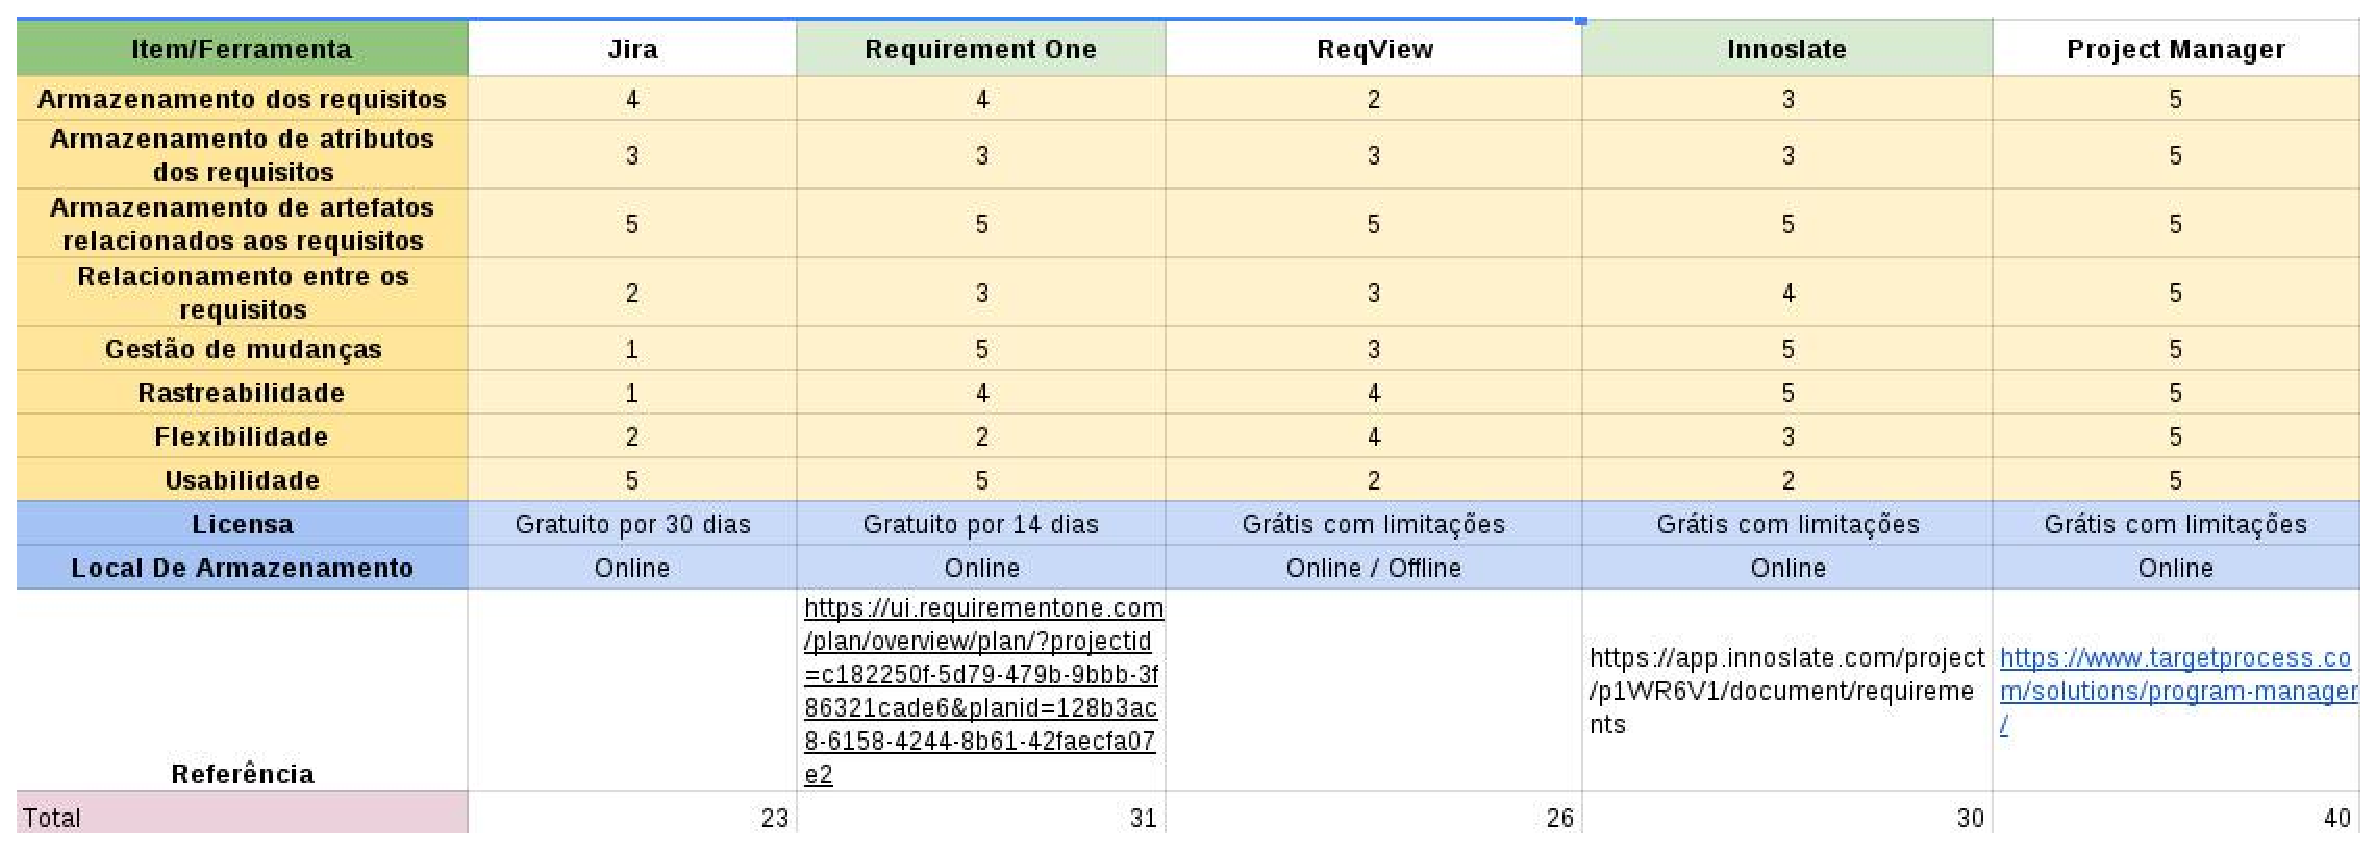
\includegraphics[keepaspectratio=true,scale=0.35]{figuras/ferramenta/ferramentas_web.eps}
      \caption{Comparação de Ferramentas Web de Gestão de Requisitos.}
      \label{fig:progama}
  \end{figure}

  Como pode ser identificado na análise, a ferramenta que melhor nos atendeu foi a "Project Manager"

  Ao acessar o Project Manager nota-se que a ferramenta foi criada exclusivamente para metodologias ágeis o que surpreendeu. A ferramenta tem um ótimo design e bem limpo.
  No lado esquerdo tem um menu com todas as opções que a ferramenta disponibiliza que são:
  \begin{enumerate}
  \item \textbf{Project e People }
  \item \textbf{Test Management }
  \item \textbf{Development Team }
  \item \textbf{Kanban Team }
  \item \textbf{Scrum Team }
  \item \textbf{Project Management }
  \item \textbf{Portifolio Management }
  \item \textbf{Dashboard }
  \end{enumerate}
  É possível criar épicos, features e historias, podendo fazer a rastreabilidade entre elas.
  A ferramenta inclui muito mais do que somente gerênciar requisitos, podendo gerência toda a equipe, projeto, tarefas, etc. O que a torna um grande potêncial para nosso uso.

  \begin{figure}[H]
    \centering
  \includegraphics[keepaspectratio=true,scale=0.3]{figuras/ferramenta/ferramenta_project_manager.eps}
    \caption{Ferramenta Project Manager - Visão Geral.}
    \label{fig:progama}
  \end{figure}


\section{Ferramenta Escolhida}

  A ferramenta Project Manager definida com o a mais adequada possui visualizações customizadas, com base nisso
  as ilustrações a seguir exemplificam uma visão geral das principais funcionalidades que serão utilizadas.


  \begin{figure}[H]
    \centering
  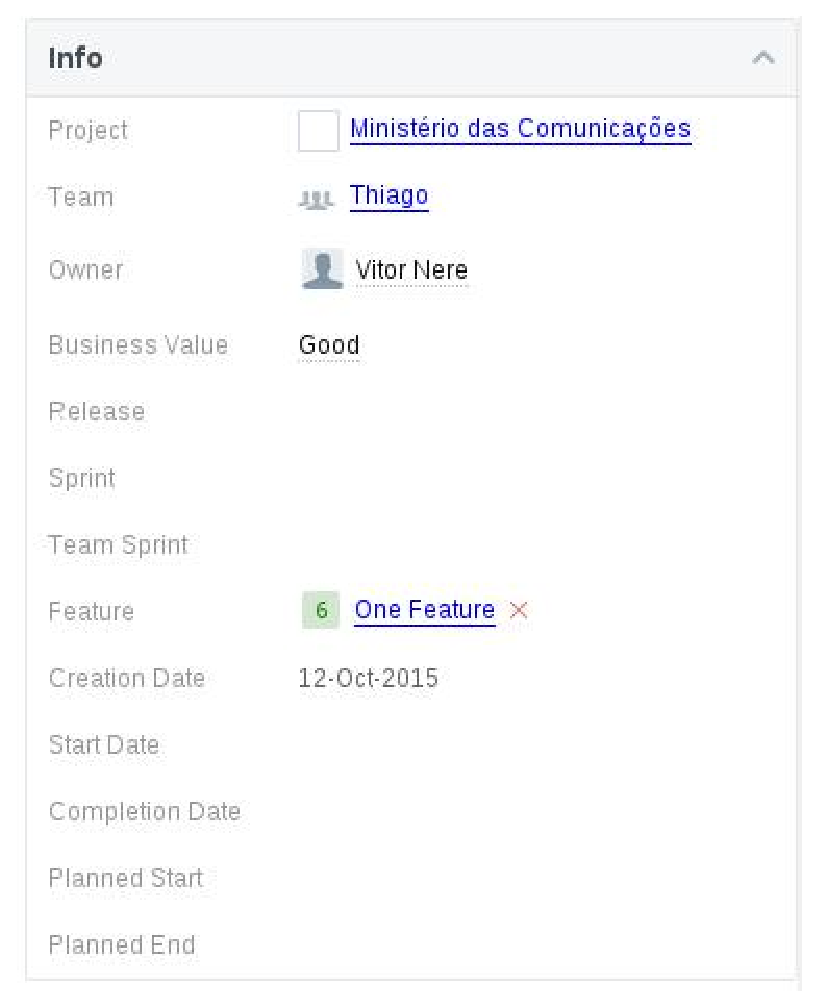
\includegraphics[keepaspectratio=true,scale=0.4]{figuras/ferramenta/pm_user_storie_2.eps}
    \caption{Ferramenta Project Manager - Visão Geral Atributos de História de Usuário.}
    \label{fig:progama}
  \end{figure}

    \begin{figure}[H]
      \centering
    \includegraphics[keepaspectratio=true,scale=0.4]{figuras/ferramenta/pm_user_storie_3.eps}
      \caption{Ferramenta Project Manager - Visão Geral Rastreabilidade Historia de Usuário.}
      \label{fig:progama}
    \end{figure}

    \begin{figure}[H]
      \centering
    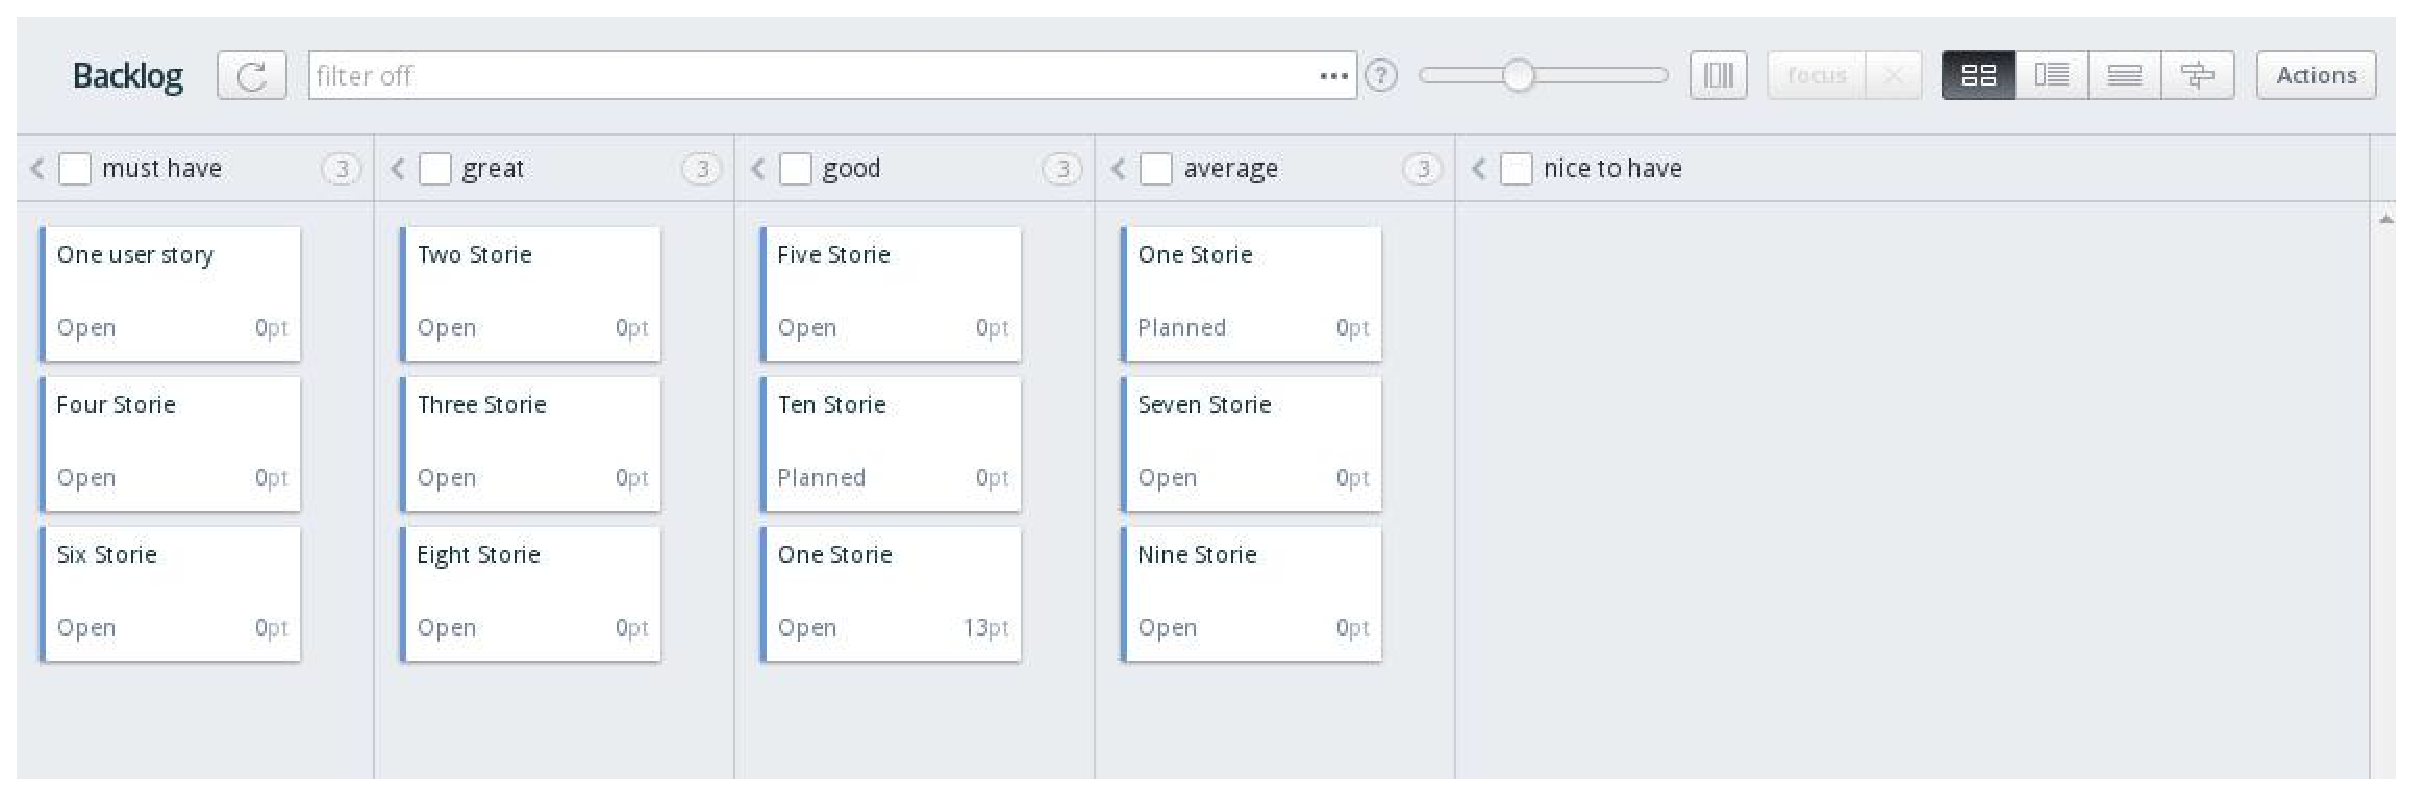
\includegraphics[keepaspectratio=true,scale=0.4]{figuras/ferramenta/pm_user_storie_4.eps}
      \caption{Ferramenta Project Manager - Visão Geral Backlog do Time.}
      \label{fig:progama}
    \end{figure}

    \begin{figure}[H]
      \centering
    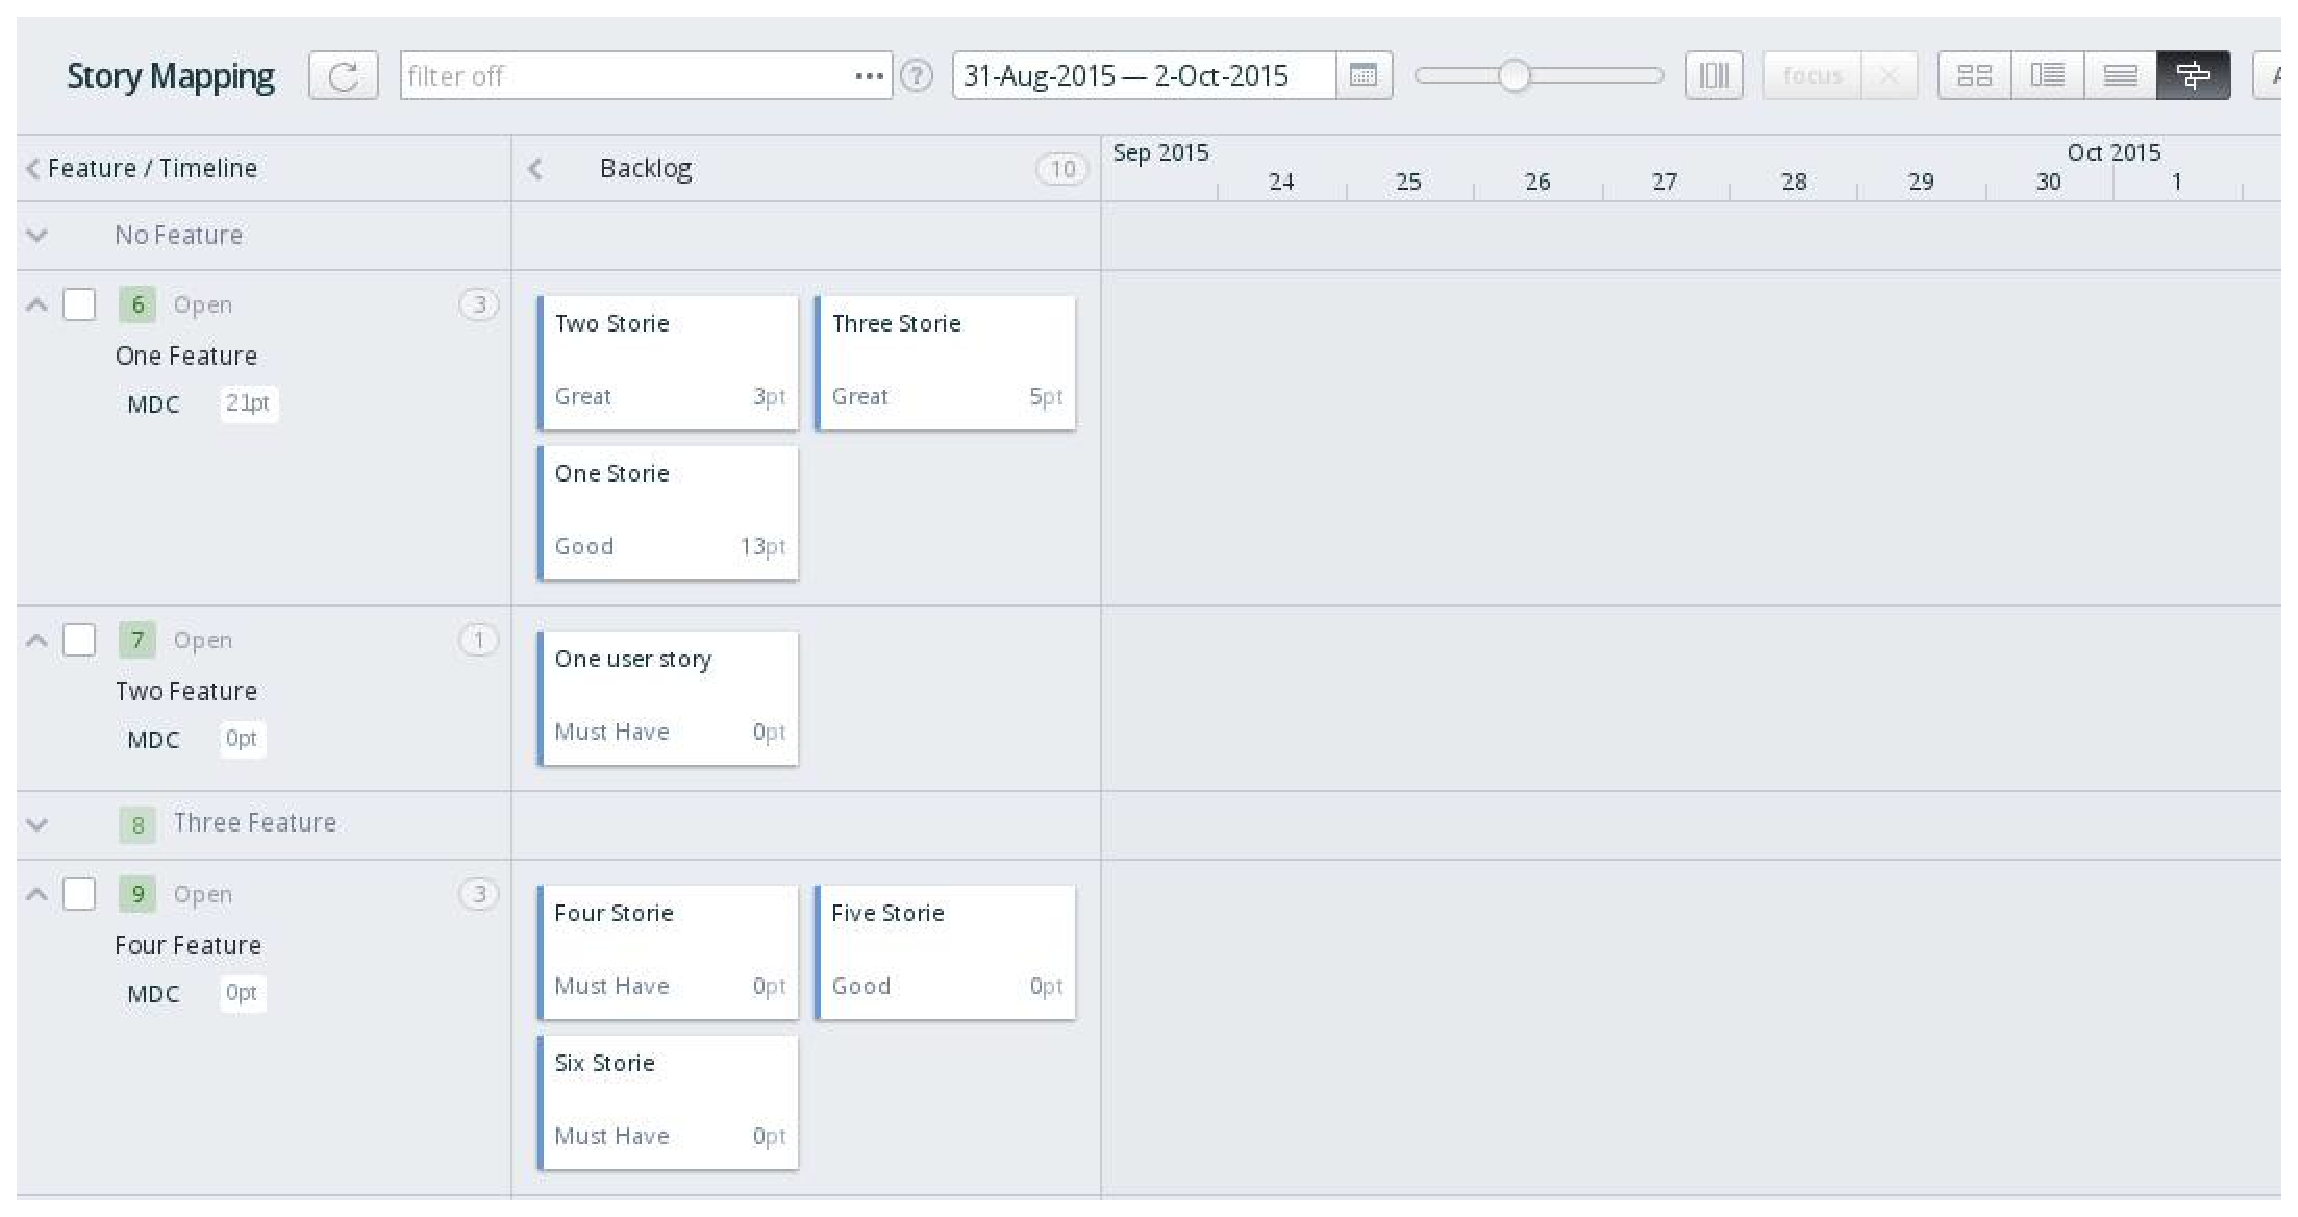
\includegraphics[keepaspectratio=true,scale=0.4]{figuras/ferramenta/pm_user_storie_5.eps}
      \caption{Ferramenta Project Manager - Visão Geral Roadmap.}
      \label{fig:progama}
    \end{figure}

    \begin{figure}[H]
      \centering
    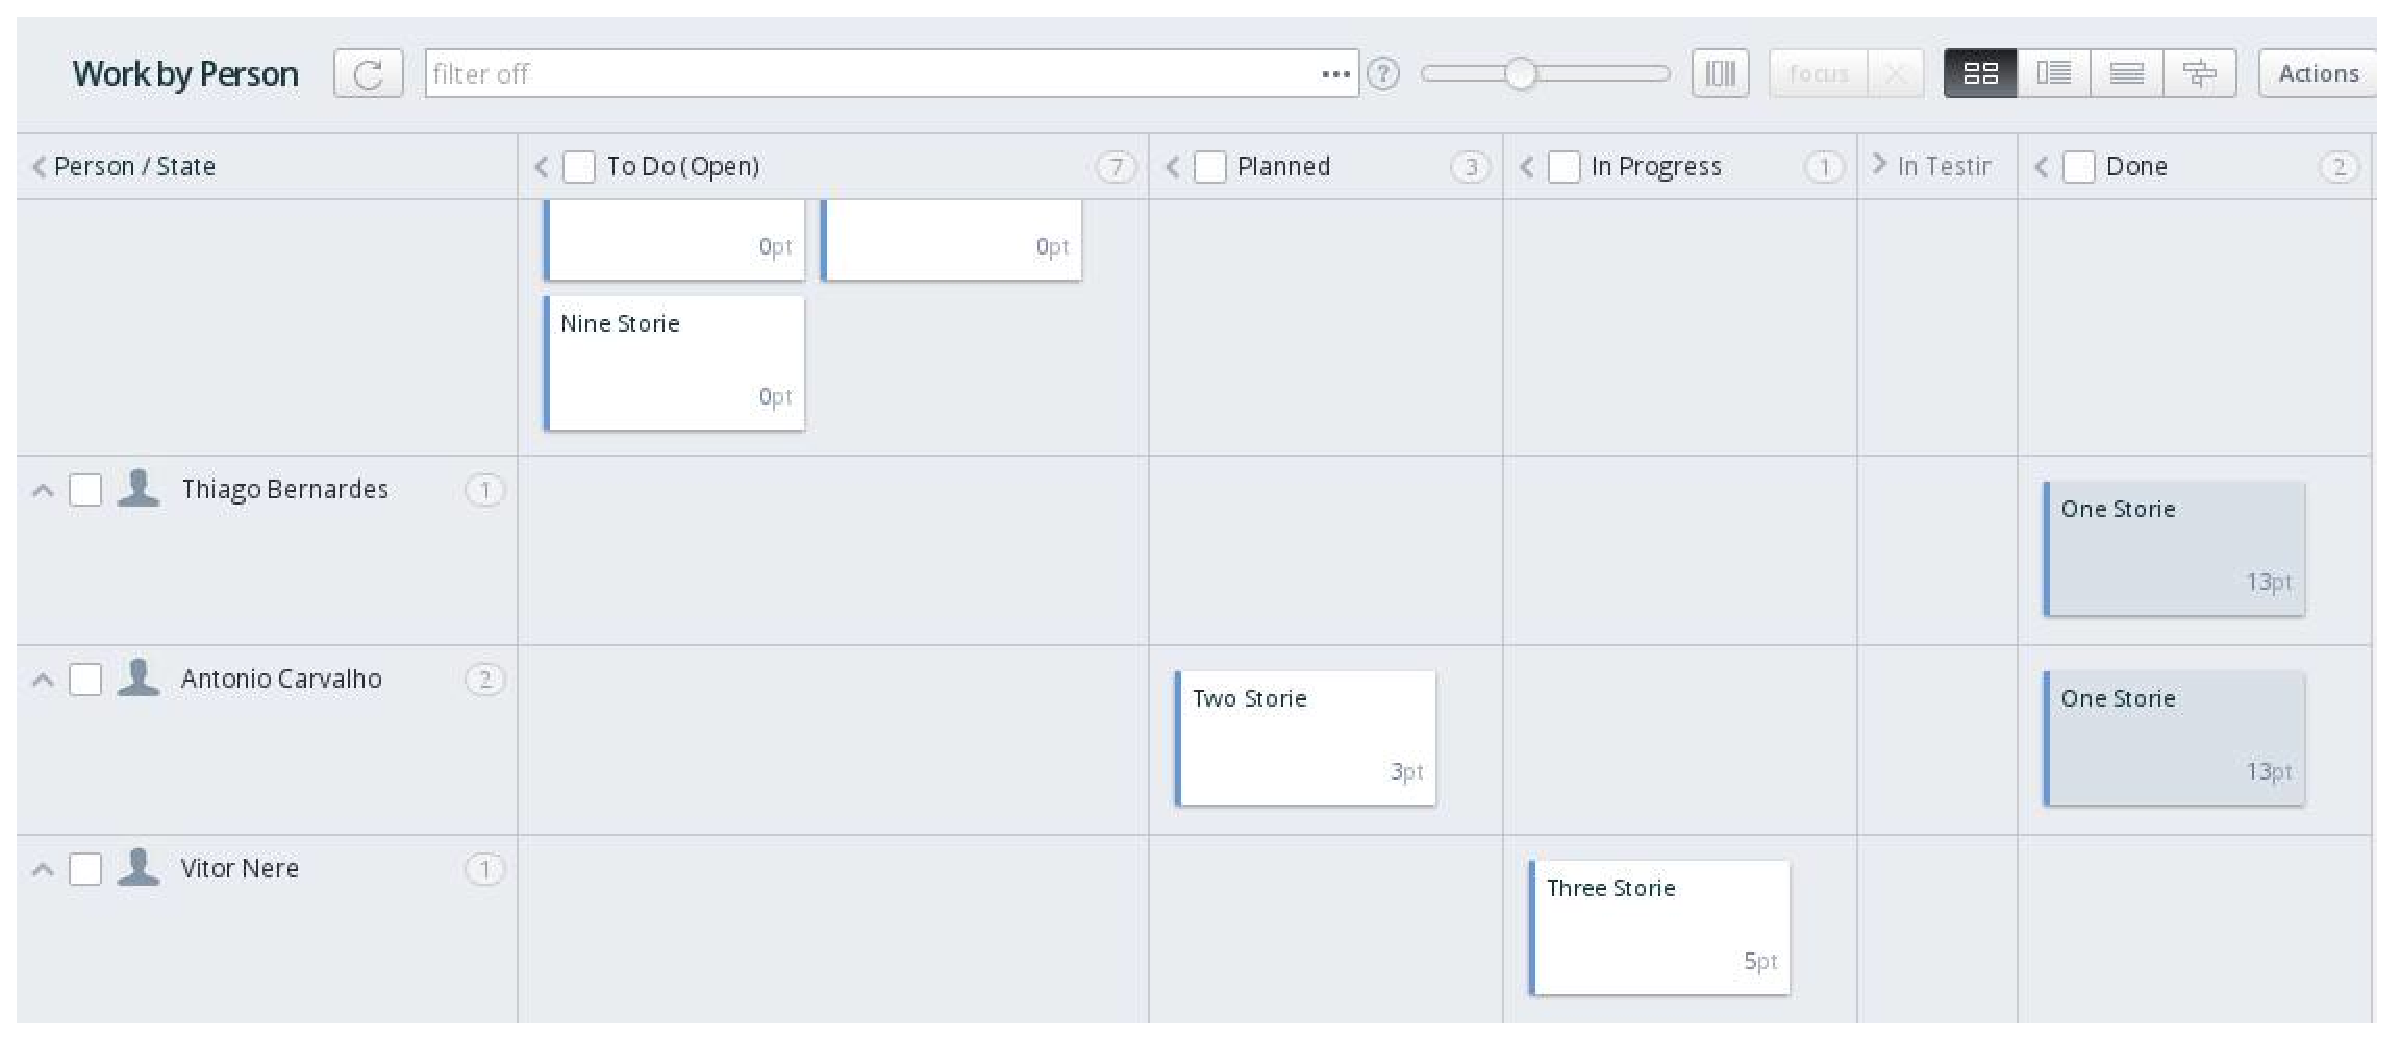
\includegraphics[keepaspectratio=true,scale=0.4]{figuras/ferramenta/pm_user_storie_6.eps}
      \caption{Ferramenta Project Manager - Atribuições e Responsáveis.}
      \label{fig:progama}
    \end{figure}
